\documentclass{article}
\usepackage[table]{xcolor}
\usepackage{tikz}
\usetikzlibrary{}
\usetikzlibrary{matrix,chains,positioning,decorations.pathreplacing,arrows}
\usetikzlibrary{positioning,calc}
\usetikzlibrary{graphs,graphs.standard,quotes}
\usepackage{pgfplots}
\pgfplotsset{compat=1.17}
\usepackage[utf8]{inputenc}
\usepackage{amsmath}
\usepackage{amssymb}

\newcommand{\jmp}[1]{[\![#1]\!]}

\begin{document}

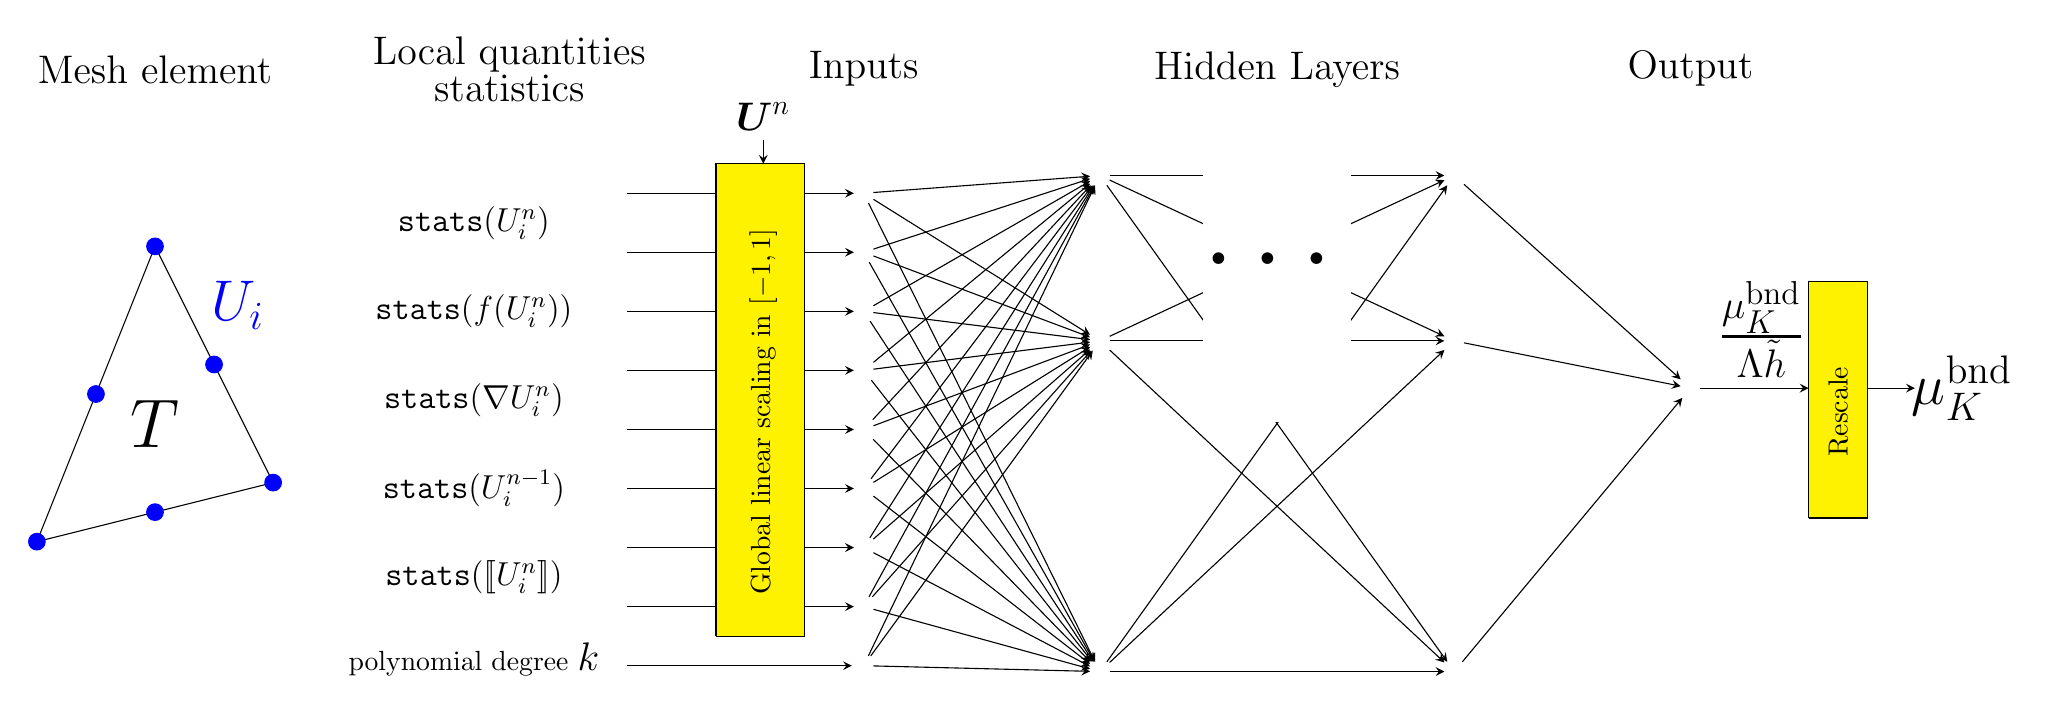
\begin{tikzpicture}[x=1.5cm, y=1.5cm, >=stealth]

\foreach \m/\l [count=\y] in {1,2,3,4,5,6,7,8,9}
  \node [every input_neuron/.try, input_neuron \m/.try] (input-\m) at (0,1.95-\y/2) {};

\foreach \m [count=\y] in {1,2,missing,3}
  \node [every neuron/.try, neuron \m/.try ] (hidden1-\m) at (2,3-\y*1.4) {};

\foreach \m [count=\y] in {1,2,missing,3}
  \node [every neuron/.try, neuron \m/.try ] (hidden2-\m) at (5,3-\y*1.4) {};

\foreach \m [count=\y] in {1}
  \node [every neuron/.try, neuron \m/.try ] (output-\m) at (7,0.8-\y) {};

\draw [<-] (input-1) -- ++(-2,0) node [above, midway] {\ };
\draw [<-] (input-2) -- ++(-2,0) node [above, midway] {\ };
\draw [<-] (input-3) -- ++(-2,0) node [above, midway] { \ };
\draw [<-] (input-4) -- ++(-2,0) node [above, midway] { \ };
\draw [<-] (input-5) -- ++(-2,0) node [above, midway] { \ };
\draw [<-] (input-6) -- ++(-2,0) node [above, midway] { \ };
\draw [<-] (input-7) -- ++(-2,0) node [above, midway] { \ };
\draw [<-] (input-8) -- ++(-2,0) node [above, midway] { \ };



\foreach \l [count=\i] in {1,2,3} {
    \ifnum \l=3
        \node [above] at (hidden1-3.north) {};
    \else
        \node [above] at (hidden1-\i.north) {};
    \fi
}

\foreach \l [count=\i] in {1,2,3} {
    \ifnum \l=3
        \node [above] at (hidden2-3.north) {};
    \else
        \node [above] at (hidden2-\i.north) {};
    \fi
}

\foreach \l [count=\i] in {1}
  \draw [->] (output-\i) -- ++(1,0)
    node [above, midway] { \ };

\foreach \i in {1,...,9}
  \foreach \j in {1,...,3}
    \draw [->] (input-\i) -- (hidden1-\j);

\foreach \i in {1,...,3}
  \foreach \j in {1,...,3}
    \draw [->] (hidden1-\i) -- (hidden2-\j);

    \foreach \i in {1,...,3}
    \foreach \j in {1}
    \draw [->] (hidden2-\i) -- (output-\j);

\node[fill=black!0,scale=4,inner xsep=0pt,inner ysep=5mm] at ($(hidden1-1)!.5!(hidden2-2)$) {$\dots$};


% labels
\node at (0,2.5)   {\Large Inputs};
\node at (3.5,2.5) {\Large Hidden Layers};
\node at (7,2.5)   {\Large Output};
\node at (-6,2.5)  {\Large Mesh element};
\node[align=center] at (-3,2.5)  {\Large Local quantities\\ \Large statistics};

% statistics
\node at (-3.3, 1.20) {\large \tt{stats}$(U_i^n)$       };
\node at (-3.3, 0.45) {\large \tt{stats}$(f(U^n_i))$ };
\node at (-3.3,-0.30) {\large \tt{stats}$(\nabla U_i^n)$};
\node at (-3.3,-1.05) {\large \tt{stats}$(U_i^{n - 1})$ }; 
\node at (-3.3,-1.80) {\large \tt{stats}$(\jmp{U^n_i})$ };

% input poly deg
\node at (-3.3, -2.5) {polynomial degree \Large $k$};
\draw [<-] (-0.1, -2.55) -- (-2.0, -2.55) node [above, midway] { \ };

% input scaling
\draw[fill=yellow] (-1.25,-2.3) -- (-0.5, -2.3) -- (-0.5, 1.7) -- (-1.25,1.7) -- (-1.25,-2.3);
\node[rotate=90] at (-0.85,-0.4) {Global linear scaling in $[-1, 1]$};
\node at (-0.85, 2.1) {\Large $\boldsymbol{U}^n$};
\draw [<-] (-0.85, 1.7) -- (-0.85, 1.9) node [above, midway] { \ };

% output rescaling
\draw[fill=yellow] (8,-1.3) -- (8.5, -1.3) -- (8.5, 0.7) -- (8,0.7) -- (8,-1.3);
\node[rotate=90] at (8.25,-0.4) {Rescale};
\node at (7.6,0.3) {\huge $\frac{\mu_K^\text{bnd}}{\Lambda \tilde{h}}$};
\node at (9.3,-0.2) {\huge $\mu_K^\text{bnd}$};
\draw [->] (8.5,-0.2) -- (8.9,-0.2) node [above, midway] { \ };

% Element T
\node at (-6,-0.5) {\Huge $T$};
\node[color=blue] at (-5.3,0.5) {\huge $U_i$};

\draw (-7,-1.5) -- (-6, 1) -- (-5, -1) -- (-7,-1.5) ;

\node[mark size=3pt,color=blue] at (-7,-1.5) {\pgfuseplotmark{*}};
\node[mark size=3pt,color=blue] at (-6, 1) {\pgfuseplotmark{*}};
\node[mark size=3pt,color=blue] at (-5, -1) {\pgfuseplotmark{*}};
\node[mark size=3pt,color=blue] at (-6.5, -0.25) {\pgfuseplotmark{*}};
\node[mark size=3pt,color=blue] at (-5.5, 0) {\pgfuseplotmark{*}};
\node[mark size=3pt,color=blue] at (-6, -1.25) {\pgfuseplotmark{*}};

\end{tikzpicture}

\end{document}